\documentclass[16pt]{article}
\usepackage[russian]{babel}
\usepackage{amsmath}
\usepackage{wrapfig}
\usepackage{floatflt}
\usepackage{graphicx}
\usepackage{fancyhdr}
\usepackage[a5paper, top=1.5cm, bottom=1.5cm, left=1.2cm, right=1.5cm]{geometry} 
\pagestyle{fancy}
\fancyhf{}
\fancyfoot[L]{\thepage}
\renewcommand{\headrulewidth}{0pt}
\renewcommand{\footrulewidth}{0pt}
\setcounter{page}{14}
\begin{document}

\begin{wrapfigure}{l}{0.3\textwidth}
  \centering
  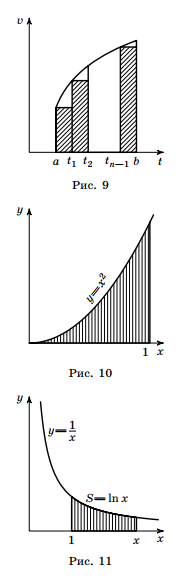
\includegraphics[width=0.35\textwidth]{Pic9-11.png}

\end{wrapfigure}
\noindentПримем для удобства $t_0 = a$, $t_n = b$. 
Тогда площадь $S$, о которой идёт речь, с любой точностью можно заменить на сумму площадей прямоугольников с нижними основаниями $[t_0, t_1], [t_1, t_2], \ldots, [t_{n-1}, t_n]$ и с высотами $v(t_0), v(t_1), \ldots, v(t_{n-1})$ (рис. 9), т. е. получаем
\[
 \approx v(t_1)(t_1 - t_0) + v(t_1)(t_2 - t_1) + \ldots + v(t_{n-1})\times(t_n - t_{n-1})\]
\[
= \sum_{k=0}^{n-1} v(t_{k}) (t_{k+1} - t_{k}) = \sum_{k=0}^{n-1} v(t_{k}) (\bigtriangleup{t_{k}}),
\]
(это сокращённое обозначение левой части).

\noindentБолее точная запись:
\[
S = \lim_{\Delta t_k \to 0 \atop n \implies \infty} \sum_{k=1}^{n} v(t_{k-1}) \Delta t_k = \lim_{\Delta t_k \to 0} \sum_{k=1}^{n} v(t_{k-1}) \Delta t_k,
\]
где $\Delta t_k = t_k - t_{k-1}$. Можно, например, брать разбиение отрезка $[a, b]$ на $n$ равных частей, так что $\Delta t_k = \frac{b - a}{n}$ и тогда условие перехода к пределу заключается просто в том, что $n \to \infty$. Но, с другой стороны, точно так же можно наращивать путь, продвигаясь в промежутке от $a$ до $b$, так как на маленьких участках $[t_k, t_{k+1}]$ скорость можно считать постоянной. Итак,
\\
\[
S = \int_a^b v(t) dt = \lim_{\Delta t_k \to 0} \sum_{k=0}^{n-1} v(t_k) \Delta t_k.
\]

\noindent Отметим соглашение о знаке площади: если кусок площади лежит под осью абсцисс, то его знак считается отрицательным, так как в этом случае $\Delta t_k > 0$, а $v(t_k) < 0$.


\\
\textbf{Пример 1.} Найдём площадь $S$ под параболой $y = x^2$ от точки $x = 0$ до точки $x = 1$ (рис. 10). Имеем:
\[
S = \int_0^1 x^2 \, dx = \set\big{ \left\frac{x^3}{3} \right]_0^1} = \frac {1}{3}.
\]

\textbf{Пример 2.} Площадь под гиперболой $y = 1/x$ от $x = 1$ до произвольного $x$ равна $\int_1^x \frac{1}{t} \, dt = \ln t \Big|_1^x = \ln x$ (рис. 11). Таков геометрический смысл натурального логарифма.
\end{document}